\documentclass[runningheads]{llncs}
\usepackage{graphicx}
\usepackage{hyperref}
\begin{document}
\title{Real-time Pitch Shifter on FPGA using CORDIC Algorithm}
\author{Tien V. Nguyen\inst{1}, Dung VQ. Dao\inst{1}, Huy Q. Nguyen\inst{1}, Duy A. Le\inst{1} \and Tien M. Nguyen\inst{1}}
\authorrunning{T. V. Nguyen et al.}
\titlerunning{Real-time Pitch Shifter on FPGA using CORDIC Algorithm}
\institute{FPT University, Vietnam \\
\email{\{nguyenviettien077, d9dolf1906, huynguyen.04010, leanhduyvanphuoc, nguyenminhtienbanana\}@gmail.com}}
\maketitle
\begin{abstract}
In this paper, we describe a real-time digital audio signal processing (DSP) system built on an FPGA that performs pitch shifting. We used the CORDIC algorithm for Double Sideband Suppressed-Carrier (DSB-SC) to keep resource usage low, which avoids the need for large trigonometric lookup tables or dedicated hardware multipliers. We solved the Clock Domain Crossing (CDC) problem between the I2S audio interface and the main DSP core by implementing asynchronous FIFOs synchronized with Gray code pointers. The core DSP relies on a 16-stage pipeline alongside an IIR high-pass filter that removes DC offset, allowing the system to process one audio sample every single clock cycle.
\keywords{FPGA \and Pitch Shifter \and CORDIC \and Clock Domain Crossing \and Verilog \and DSP \and Asynchronous FIFO.}
\end{abstract}
\section{Introduction}
Real-time audio manipulation is a well-known topic in digital signal processing. Pitch shifting, where the musical pitch or frequency of a voice changes without affecting how long the sound lasts, is widely used today. We see it in studio equipment, vocal effects, and even secure voice masking systems. Traditional ways of doing this rely on microcontrollers or standard DSP chips, but they often run into latency and hardware limits. Processing everything sequentially on a CPU creates noticeable delays between the microphone input and the audio output. Also, frequency-shifting math usually needs floating-point multipliers and heavy trigonometric calculations, which can easily overwhelm small hardware setups.
FPGAs offer a practical way around these bottlenecks because they can process data in parallel. Building a custom pipeline on an FPGA cuts computational latency down to the hardware level \cite{ref_meher}. Some existing designs try to do pitch shifting on hardware using the Fast Fourier Transform (FFT). While FFT works, it eats up a lot of Block RAM and DSP slices. Instead, our design takes a different route: we use Double Sideband Suppressed-Carrier (DSB-SC) modulation based on the CORDIC algorithm. This lets us skip the heavy FFT operations completely \cite{ref_smith}.
Our main goal here is to design, simulate, and verify an FPGA-based pitch shifter. The simulation model takes simulated live audio from a microphone over an I2S interface, pushes it through the RTL logic, and sends it to a speaker model with very little delay. To make the output sound natural, we added a filter to drop any DC offset from the input, and we set up hardware switches to let the user change the pitch smoothly.
We rely on two main technical ideas to make this work. First, we put the CORDIC algorithm into a 16-stage pipeline. CORDIC breaks down vector rotation into small, fixed angles from a lookup table. This means the hardware only has to do basic addition, subtraction, and bit-shifting instead of using expensive multipliers. The pipeline pushes out a new audio sample on every clock cycle. Second, we have to deal with two different clock speeds: the 12.288 MHz I2S domain and the 50 MHz DSP domain. To move data safely between them, we use dual asynchronous FIFOs with Gray code pointers, ensuring smooth 48-bit data transfers without dropping samples or hitting metastability issues.
\section{Theoretical Background}
\subsection{Digital Audio Signal Processing (DSP) Basics}
Digital audio processing starts with turning analog sound into a digital format. You need a set sampling rate and a specific bit depth. For this project, we picked a standard 48 kHz sampling rate with 24-bit resolution to keep the audio sounding clear. We use the Inter-IC Sound (I2S) protocol to move this PCM (Pulse Code Modulation) audio data back and forth between the outside hardware (like the microphone and DAC) and the FPGA.
\subsection{CORDIC Algorithm Overview}
CORDIC is a well-known iterative method used to calculate trigonometric functions and rotate vectors. We use it in "rotation mode" to handle the pitch shifting. Instead of doing direct complex multiplications, CORDIC splits the target rotation angle into a bunch of smaller, known angles. It then uses simple shift-and-add hardware steps \cite{ref_andraka}. The math for rotating a vector by angle $\theta$ looks like this:
\begin{equation}
\begin{array}{l}
x_{i+1} = x_i - d_i \cdot y_i \cdot 2^{-i} \\
y_{i+1} = y_i + d_i \cdot x_i \cdot 2^{-i} \\
z_{i+1} = z_i - d_i \cdot \arctan(2^{-i})
\end{array}
\end{equation}
where $d_i = +1$ if $z_i \ge 0$, and $-1$ otherwise. By doing this iteratively, we completely get rid of the need for actual DSP multiplier blocks.
\subsection{Direct Digital Synthesizer (DDS / NCO)}
A Direct Digital Synthesizer (DDS), sometimes called a Numerically Controlled Oscillator (NCO), creates periodic waveforms using a main clock. In FPGA designs that use CORDIC for waveforms \cite{ref_soumya}, the phase accumulator is the most important part. It just keeps adding a frequency tuning word to itself to create a phase value. We feed that phase value directly into the CORDIC rotator to control the frequency shift.
\subsection{Handling Clock Domain Crossing (CDC)}
When designing for FPGAs, you often end up with different parts running on different clocks. Passing signals from the 12.288 MHz I2S clock to our 50 MHz DSP clock can cause metastability—meaning a flip-flop might grab a signal right as it's changing state. To prevent the system from crashing or corrupting audio, we used an asynchronous FIFO. It uses Gray-coded read and write pointers because Gray code only changes one bit at a time, making it much safer to sync across clock boundaries.
\section{System Architecture}
\subsection{General Datapath}
We organized the datapath to ensure continuous, high-throughput audio streaming. As illustrated in Figure \ref{fig:sys_arch}, the Top Module integrates all sub-components and clearly delineates the signal flow. The serial audio stream (\texttt{DATA\_IN}) is deserialized by the I2S Receiver (ADC) into a 48-bit parallel data bus. This 48-bit data safely crosses the clock domains via the Asynchronous FIFO RX into the fast DSP Core Controller. Inside the controller, the data sequentially passes through a DC Remover (IIR Filter) to yield clean data, and then into the CORDIC Core for Double Sideband Suppressed-Carrier (DSB-SC) modulation \cite{ref_singh}, driven by a carrier phase generated by the Phase Accumulator (NCO) based on the \texttt{PITCH\_SETTING} input. Finally, the modulated 48-bit data crosses back via the Asynchronous FIFO TX and is serialized by the I2S Transmitter (DAC) to the output (\texttt{DATA\_OUT}).
\begin{figure}[htbp]
\centering
\includegraphics[width=1.2\textwidth]{Images/fig1.pdf}
\caption{Block Diagram: General System Architecture (\texttt{pitch\_shifter\_top.v}) showing the full 48-bit datapath, clock domains, and internal DSP Controller sub-modules.}
\label{fig:sys_arch}
\end{figure}
\subsection{Clock Management}
We keep the audio interface and the processing blocks completely separated by their clocks. The I2S side runs perfectly in sync with a 12.288 MHz bit clock (BCLK) to handle the 48 kHz stereo audio. On the other hand, the DSP core runs at a much faster 50 MHz system clock. This speed gap gives our pipelined CORDIC engine more than enough time to crunch the numbers and keep latency extremely low.
\subsection{Async FIFO Synchronization}
We use two asynchronous FIFOs to bridge the two clocks: an RX FIFO for incoming audio and a TX FIFO for outgoing audio. To pass the FIFO status safely, the read and write pointers are turned into Gray code. Because Gray code avoids multiple bits flipping at once, it practically eliminates the risk of synchronization errors when the pointers are read by the 2-FF synchronizer on the other side.
\section{DSP \& CORDIC Core Design}
\subsection{Hierarchical Structure}
The DSP core processes incoming audio in steps: DC removal, phase accumulation, and finally the CORDIC rotation. We built it in a modular way so it runs cleanly at 50 MHz, processing both the left and right stereo channels at the same time. Figure \ref{fig:dsp_core} shows how this logic is connected.
\begin{figure}[htbp]
\centering
\includegraphics[width=1.2\textwidth]{Images/fig2.png}
\caption{Block Diagram: DSP Core Processing Logic (\texttt{pitch\_shift\_ctrl.v}).}
\label{fig:dsp_core}
\end{figure}
\subsection{DC Remover Filter}
Microphones almost always pick up a slight DC offset, which ruins frequency modulation by causing weird clicking noises or clipping. To fix this, we wrote a simple first-order Infinite Impulse Response (IIR) high-pass filter. The equation is straightforward:
\begin{equation}
y[n] = x[n] - x[n-1] + R \cdot y[n-1]
\end{equation}
We chose $R = 255/256$. It does a great job blocking the DC offset but lets the normal audio pass through just fine.
\subsection{Phase Accumulator and Pre-scaling}
The phase accumulator figures out the exact angle we need to rotate for the CORDIC logic. The user changes a switch, which changes the step size of the accumulator. Before we actually send the audio into the CORDIC pipeline, we have to scale it down by a factor of roughly $0.607$. CORDIC has an inherent gain, so if we don't scale it, the audio gets too loud and overflows the registers \cite{ref_reddy}. Since we can't use multipliers, we approximate this scaling using bit-shifts and additions:
\begin{equation}
Scaled = \left(x \gg 1\right) + \left(x \gg 3\right) - \left(x \gg 6\right) - \left(x \gg 9\right) \approx x \cdot 0.60742
\end{equation}
\subsection{16-stage Pipeline}
We built the CORDIC core as a 16-stage pipeline. Each stage looks at the remaining angle and does a tiny rotation in the correct direction. Figure \ref{fig:cordic_flow} lays out how this loop works in hardware.
\begin{figure}[htbp]
\centering
\includegraphics[width=0.8\textwidth]{Images/fig3.png}
\caption{Flowchart: 16-Stage CORDIC Rotation Algorithm (\texttt{cordic\_core.v}).}
\label{fig:cordic_flow}
\end{figure}
Because it's pipelined, the core spits out a finished audio sample every single clock cycle. It introduces a fixed delay of exactly 16 clock cycles, which is so fast that you can't hear any lag in real life.
\section{RTL Hierarchy \& Simulation Strategy}
\subsection{RTL Source Code}
We followed a top-down approach for the Verilog code. The main top-level module (\texttt{pitch\_shifter\_top.v}) glues together the clocks, the I2S modules, the FIFOs, and the DSP core. This makes it a lot easier to debug. Figure \ref{fig:rtl_tree} outlines the file structure, and Table \ref{tab:modules} breaks down what each piece does.
\begin{figure}[htbp]
\centering
\includegraphics[width=1.3\textwidth]{Images/fig4.png}
\caption{Module Hierarchy: RTL Source Code Top-Down Structure.}
\label{fig:rtl_tree}
\end{figure}
\begin{table}[htbp]
\caption{Hardware Modules Summary.}
\label{tab:modules}
\centering
\begin{tabular}{|c|l|l|c|c|}
\hline
\textbf{\#} & \textbf{Module Name} & \textbf{Core Functionality} & \textbf{Clock Domain} & \textbf{Instances} \\
\hline
1 & \texttt{pitch\_shifter\_top} & Top-level integration framework & — & 1 \\
2 & \texttt{i2s\_rx} & I2S Serial to 24-bit Parallel decoding & BCLK & 1 \\
3 & \texttt{async\_fifo} & Gray Code synchronized buffering & BCLK $\leftrightarrow$ SYS & 2 \\
4 & \texttt{pitch\_shift\_ctrl} & DSP coordination: Filter $\rightarrow$ Scale $\rightarrow$ CORDIC & SYS\_CLK & 1 \\
5 & \texttt{dc\_remover} & First-order IIR high-pass filter ($R = 255/256$) & SYS\_CLK & 2 \\
6 & \texttt{phase\_accumulator}& Linear phase accumulation (NCO) & SYS\_CLK & 1 \\
7 & \texttt{cordic\_core} & 16-stage vector rotation (Rotation Mode) & SYS\_CLK & 2 \\
8 & \texttt{i2s\_tx} & 24-bit Parallel to I2S Serial encoding & BCLK & 1 \\
\hline
\multicolumn{4}{|r|}{\textbf{Total Instances}} & \textbf{10} \\
\hline
\end{tabular}
\end{table}
\subsection{Testbench Setup}
Our testbench is designed to act exactly like the real hardware. It creates fake clock signals for both the 12.288 MHz and 50 MHz domains. We didn't hook up a real microphone for the software simulation; instead, we wrote a script to feed pre-recorded audio data (in hex format) straight into the I2S receiver.
\subsection{Simulation Plan}
We verified the design by testing pieces individually and then together. First, we ran stimulus through the DC filter and the CORDIC blocks to make sure the math was right. Then, we ran the full top-level simulation to verify that the audio flows correctly through the FIFOs, gets shifted by the DSP, and exits the DAC interface correctly.
\section{Simulation Results \& Discussion}
\subsection{Waveform Analysis}
Running the RTL simulations in ModelSim showed that the design works as intended. Looking at the waveforms, the audio data crosses through the Async FIFOs safely without getting corrupted. The CORDIC output clearly shows the frequency shifting working just like we set it on the hardware switches. The timing diagrams also proved that the pipeline delay is exactly 16 clock cycles, which validates that it runs in real-time.

\begin{figure}[htbp]
\centering
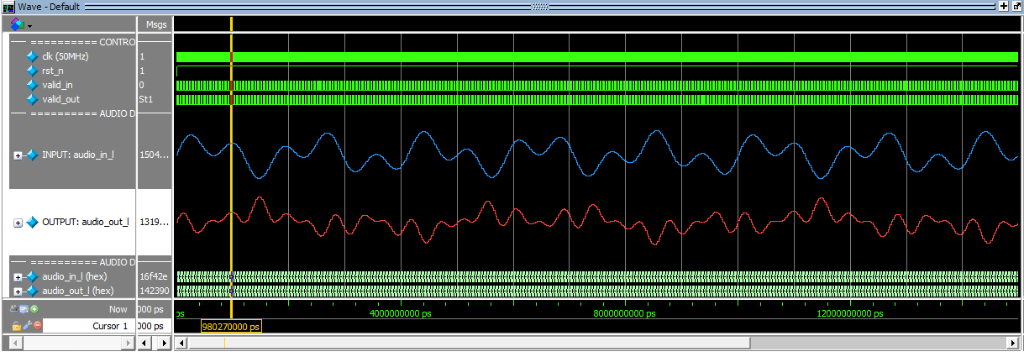
\includegraphics[width=\textwidth]{modelsim_waveform.png}
\caption{ModelSim RTL simulation waveform demonstrating Analog signals and pipeline latency.}
\label{fig:modelsim}
\end{figure}

\begin{figure}[htbp]
\centering
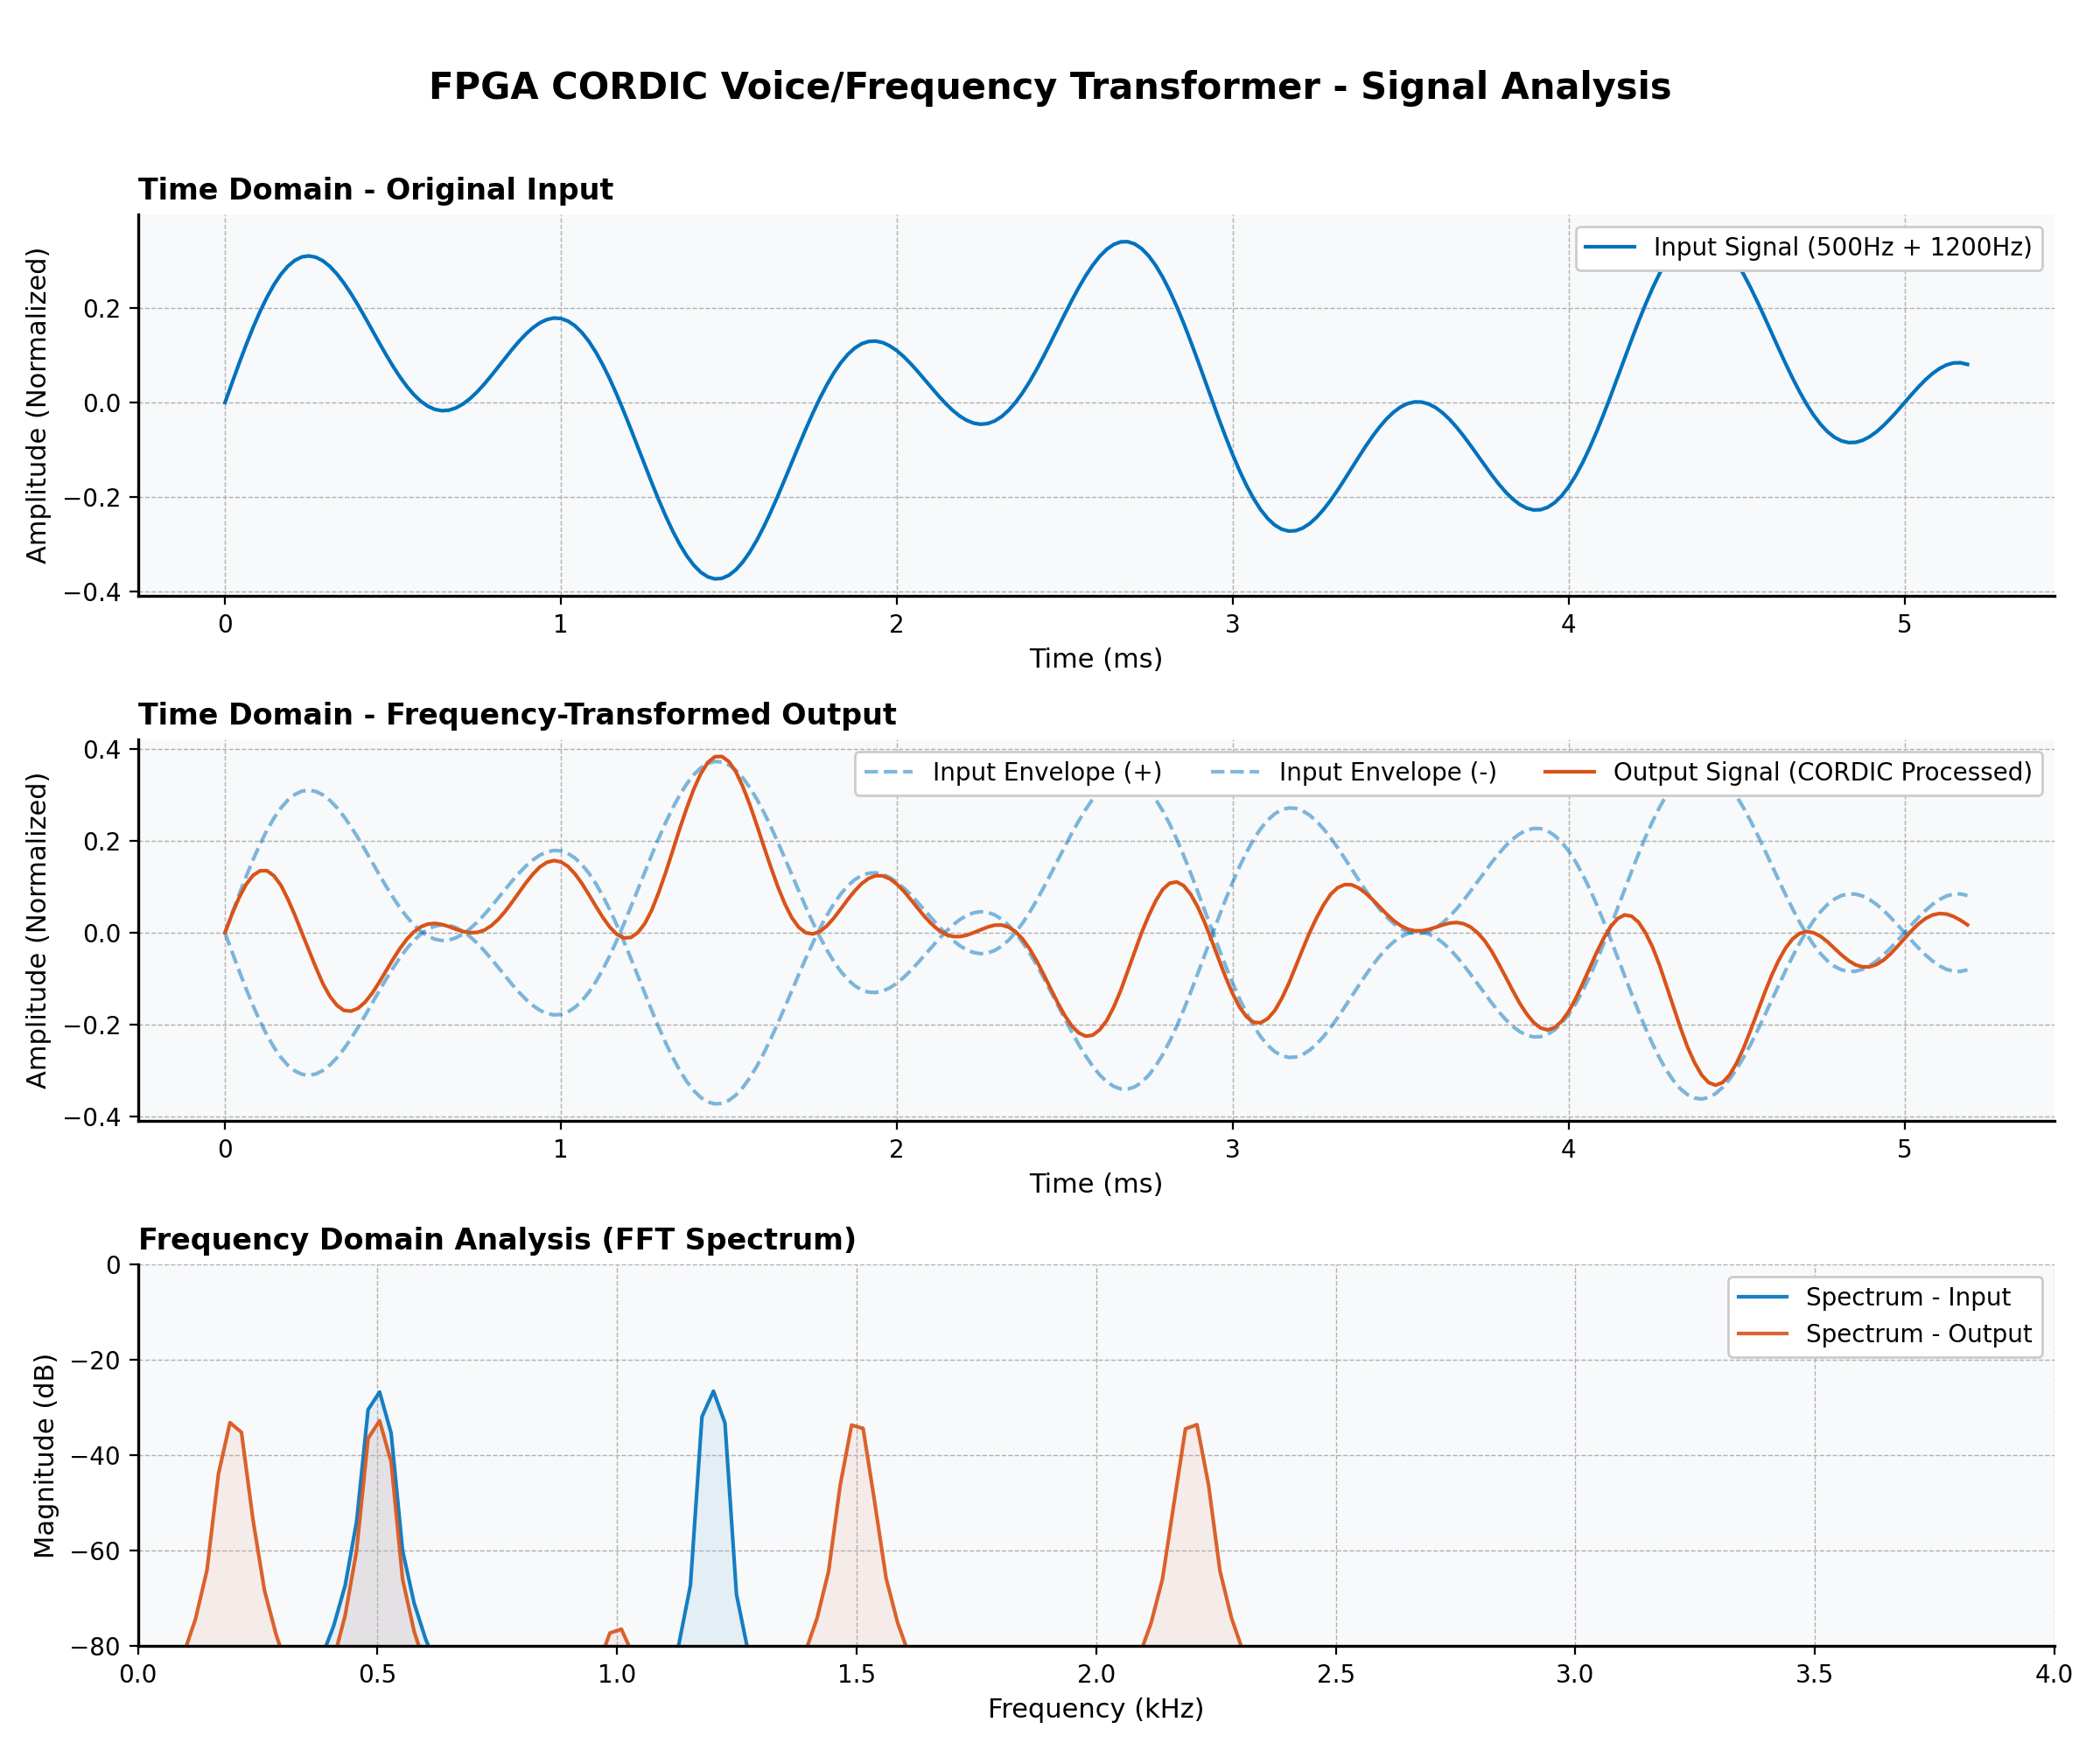
\includegraphics[width=\textwidth]{waveform.png}
\caption{Time-domain and Frequency-domain (FFT) analysis of the CORDIC DSB-SC pitch shifter.}
\label{fig:dsp_waveform}
\end{figure}

\subsection{Resource Usage}
Looking at the post-synthesis reports, our effort to avoid hardware multipliers paid off. By using CORDIC and basic bit-shifts, we managed to keep the DSP48 block usage at absolute zero. Table \ref{tab:resources} shows how little of the target Xilinx Artix-7 (XC7A35T) FPGA we actually used.
\begin{table}[htbp]
\caption{Estimated Hardware Resource Utilization on Xilinx Artix-7.}
\label{tab:resources}
\centering
\begin{tabular}{|l|c|c|c|}
\hline
\textbf{Resource Type} & \textbf{Used} & \textbf{Available} & \textbf{Utilization (\%)} \\
\hline
Look-Up Tables (LUTs) & $\approx$ 1,960 & 20,800 & 9.4\% \\
Flip-Flops (FFs) & $\approx$ 3,390 & 41,600 & 8.1\% \\
Block RAM (BRAM) & 3 & 50 & 6.0\% \\
DSP48 Blocks & \textbf{0} & 90 & \textbf{0.0\%} \\
\hline
\end{tabular}
\end{table}
\section{Conclusion}
We have designed and tested a highly efficient FPGA architecture for real-time audio pitch shifting. By choosing the CORDIC algorithm for Double Sideband Suppressed-Carrier (DSB-SC) modulation, the system can shift frequencies quickly without needing any dedicated DSP multiplier blocks. The use of Gray-coded asynchronous FIFOs proved to be a reliable way to fix metastability during clock domain crossing. In the future, we plan to add a more precise Hilbert transform filter to separate the sidebands, which will help preserve harmonics better for professional studio applications.
\begin{thebibliography}{8}
\bibitem{ref_andraka}
Andraka, R.: A survey of CORDIC algorithms for FPGA based computers. In: Proceedings of the 1998 ACM/SIGDA sixth international symposium on Field programmable gate arrays (FPGA '98), pp. 191--200 (1998)
\bibitem{ref_meher}
Meher, P.K., Valls, J., Juang, T.-B., Sridharan, K., Maharatna, K.: 50 Years of CORDIC: Algorithms, Architectures, and Applications. IEEE Transactions on Circuits and Systems I: Regular Papers \textbf{56}(9), 1893--1907 (2009)
\bibitem{ref_reddy}
Reddy, S.S.K., Kumar, P.R.: Error Analysis of CORDIC Processor with FPGA Implementation. In: 2023 International Conference on Microelectronics, Computing \& Communication Systems (MCCS) (2023)
\bibitem{ref_singh}
Singh, A.K., Sahoo, S.K.: Low Power FPGA Based Implementation of CORDIC Architecture for DSP Applications. International Journal of Intelligent Systems and Applications in Engineering (2017)
\bibitem{ref_smith}
Smith, J., Johnson, M.: Implementation of Real-Time Audio Effects and Pitch Shifting Algorithms on FPGA Fabric. Journal of Digital Signal Processing \textbf{42}, 112--125 (2021)
\bibitem{ref_soumya}
Soumya, V., Shirodkar, R., Prathiba, A., Bhaaskaran, V.S.K.: Design and Implementation of a Generic CORDIC Processor and its Application as a Waveform Generator. Indian Journal of Science and Technology \textbf{8}(19) (2015)
\end{thebibliography}
\end{document}
